\documentclass[class=book, crop=false, oneside, 12pt]{standalone}
\usepackage{standalone}
\usepackage{amsmath}
\usepackage{../../style}
\graphicspath{{./assets/images/}}

% arara: pdflatex: { synctex: yes, shell: yes }
% arara: latexmk: { clean: partial }
\begin{document}

\chapter{Lavoro elettrico, Potenziale elettrostatico}

\section{Lavoro della forza elettrica, tensione, potenziale}

La formula che esprime la forza subita da una carica \(q_0\) in un campo elettrostatico, è valida quando le cariche che generano il campo sono fisse e costanti e la carica \(q_0\) è a sua volta fissa oppure si muove senza però perturbare la distribuzione delle cariche sorgenti (da qui il termine \emph{elettrostatico}).

\subsection{Campo elettromotore}

Però possiamo dire più in generale che quando su una carica \(q_0\) agisce una forza F di qualsiasi natura, non necessariamente elettrostatica, ma ad esempio dovuta a processi chimici o ad azioni meccaniche, o altre cause, possiamo definire sempre un campo elettrico \(E\), che si indica anche col nome di campo elettromotore:
\begin{equation} \label{campo_elettromotore}
    \overrightarrow{E} = \frac{\overrightarrow{F}}{q_0} \implies \overrightarrow{F} = q_0 \overrightarrow{E}
\end{equation}
Formalmente: \emph{la forza che agisce su una carica elettrica, che come tale prende il nome di forza elettrica, si esprime sempre come prodotto della carica per un certo campo elettrico}.

\subsection{Lavoro}

Il lavoro della forza \(\overrightarrow{F}\) per uno spostamento \(d \overrightarrow{s}\) della carica \(q_0\) è dato da:
\begin{equation}
    d W = \overrightarrow{F} \cdot d \overrightarrow{s} = q_0 \overrightarrow{E} \cdot d \overrightarrow{s} = q_0 E \cos \theta ds = q_0 E_s d s
\end{equation}
dove \(\theta\) è l'angolo tra il campo elettrico \(\overrightarrow{E}\) e lo spostamento \(d \overrightarrow{s}\) e \(E_s\) la componente di \(\overrightarrow{E}\) lungo \(d \overrightarrow{s}\).

Per uno spostamento finito dalla posizione \(A\) alla posizione \(B\) lungo un percorso \(C_1\) il lavoro si ottiene suddividendo il percorso in una serie infinita di segmenti infinitesimi \(d \overrightarrow{s}_i\), calcolando per ognuno di essi il lavoro \(dW_i\).
La somma diventa:
\begin{equation} \label{lavoro_elettrostatico}
    W_1 = \int_{C_1} d W_1 = \int_{C_1} \overrightarrow{F} \cdot d \overrightarrow{s} = q_0 \int_{C_1} \overrightarrow{E} \cdot d \overrightarrow{s}
\end{equation}
dove \(d \overrightarrow{s}\) è un vettore elementare tangente alla curva, e l'ultimo integrale è l'integrale di linea del campo \(\overrightarrow{E}\) lungo \(C_1\).

\begin{figure}[h]
    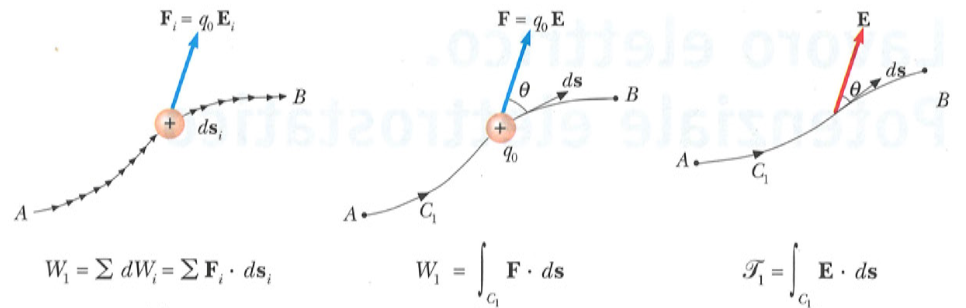
\includegraphics[scale=0.6]{lavoro_tensione_elettrostatica.png}
    \centering
    \caption{}
\end{figure}

\subsection{Tensione elettrica}

Il rapporto \(W_1 / q_0\) tra il lavoro compiuto dalla forza \(\overrightarrow{F}\) nello spostamento della carica \(q_0\) da \(A\) a \(B\) lungo il percorso \(C_1\), e il valore della carica, definisce la \emph{tensione elettrica tra i due punti \(A\) e \(B\) relativa al percorso \(C_1\)}:
\begin{equation}
    \mathcal{F} \left(A \rightarrow B \text{ lungo } C_1\right) = \int_{C_1} \overrightarrow{E} \cdot d \overrightarrow{s}
\end{equation}
Se considero un altro percorso \(C_2\) trovo un lavoro diverso e quindi un \emph{diverso valore della tensione elettrica}.
\begin{equation*}
    \mathcal{F} \left(A \rightarrow B \text{ lungo } C_1\right) \neq \mathcal{F} \left(A \rightarrow B \text{ lungo } C_2\right)
\end{equation*}

\subsection{Lavoro in un percorso chiuso}

Per un percorso chiuso \(C\) formato dal percorso \(C_1\) da \(A\) a \(B\) e dal percorso \(-C_2\) da \(B\) ad \(A\), il lavoro risulta:
\begin{equation*}
    W = \oint_{C} \overrightarrow{F} \cdot d \overrightarrow{s} = \int_{C_1} \overrightarrow{F} \cdot d \overrightarrow{s} + \int_{C_2} \overrightarrow{F} \cdot d \overrightarrow{s} = \int_{C_1} \overrightarrow{F} \cdot d \overrightarrow{s} - \int_{-C_2} \overrightarrow{F} \cdot d \overrightarrow{s} = W_1 - W_2
\end{equation*}
Ottengo quindi che \emph{in generale il lavoro per un percorso chiuso è diverso da zero}. Inserendo (\ref{campo_elettromotore})
\begin{equation}
    W = \oint_{C} \overrightarrow{F} \cdot d \overrightarrow{s} = q_0 \oint_{C} \overrightarrow{E} \cdot d \overrightarrow{s} = q_0 \mathcal{E}
\end{equation}
Il lavoro per spostare una carica lungo il percorso chiuso \(C\) è dato dal prodotto della carica per la circuitazione del campo elettrico lungo \(C\).

\subsection{Forza elettromotrice}

L'integrale 
\begin{equation}
    \mathcal{E} = \oint_C \overrightarrow{E} \cdot d \overrightarrow{s}
\end{equation}
che esprime il rapporto tra lavoro compiuto sulla carica e la carica stessa per lo spostamento \(C\) si definisce \emph{forza elettromotrice (f.e.m. del campo elettrico)} relativa al percorso \(C\).
\begin{figure}[h]
    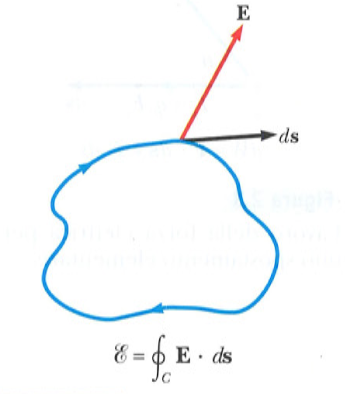
\includegraphics[scale=0.5]{circuitazione.png}
    \centering
    \caption{}
\end{figure}
Essa è in generale diversa da zero e dipende dalle caratteristiche del campo e dal percorso \(C\) scelto; malgrado il nome, \emph{non è una forza}.

\subsection{Forze conservative}
Per le forze dette \emph{conservative} il lavoro compiuto nello spostamento di un punto da A a B è funzione soltanto della posizione di partenza e di quella di arrivo e non del cammino seguito.

Ne deriva che il lavoro lungo un qualsiasi percorso chiuso è nullo, ovvero (nel nostro caso della forza elettrica) che la circuitazione di una forza conservativa è nulla.

Non si verifica in natura che qualsiasi \emph{forza elettrica} sia conservativa; questo è però il caso delle forze \emph{elettrostatiche}, ottengo quindi che \emph{il campo elettrostatico è conservativo} (dimostrazione in seguito).

\subsection*{Differenza di potenziale}

Non dipendendo dal percorso effettivamente seguito l'integrale che compare in (\ref{lavoro_elettrostatico}) può sempre essere espresso come differenza dei valori di una funzione delle coordinate, chiamata potenziale elettrostatico: 
\begin{equation} \label{differenza_di_potenziale}
    V_B - V_A = \Delta V = - \int_A^B \overrightarrow{E} \cdot d \overrightarrow{s}
\end{equation}
In realtà è la differenza di potenziale (d.d.p.) elettrostatico tra il punto \(B\) e il punto \(A\) ad essere definita da (\ref{differenza_di_potenziale}) e ciò vuol dire che il potenziale elettrostatico in un punto è determinato a meno di una costante additiva.

Inserendo la differenza di potenziale nella definizione di lavoro:
\begin{equation}
    W_{AB} = -q_0 \left(V_B - V_A\right) = -q_0 \Delta V
\end{equation}

\subsection*{Energia potenziale}

Ricordiamo che ad ogni forza conservativa è associata una determinata \emph{energia potenziale} e che il lavoro della forza  conservativa \emph{è pari all'opposto della variazione della corrispondente energia potenziale}.
\begin{equation*}
    W_{AB} = - \Delta U_e = - \left[U_e (B) - U_e (A)\right]
\end{equation*}
segue l'ugualianza:
\begin{equation}
    \Delta U_e = q_0 \Delta V
\end{equation}
La \(U_e\) prende il nome di energia potenziale elettrostatica, risulta proporzionale al potenziale elettrostatico e anch'essa definita a meno di una costante additiva. 

Segue che per un qualsiasi percorso chiuso nella regione in cui è definito il campo elettrostatico \(E\), essendo la differenza di potenziale nulla in quanto \(A \equiv B\), valgono le relazioni:
\begin{equation}
    \mathcal{E} = \oint \overrightarrow{E} \cdot d \overrightarrow{s} = 0 \ , \ W = q_0 \mathcal{E} = 0
\end{equation}
In un campo elettrostatico la forza elettromotrice è uguale a zero, ovvero è nullo il lavoro compiuto dalla forza elettrostatica per qualsiasi percorso ciclico.

\section{Calcolo del potenziale elettrostatico}

\subsection*{Campo generato da una carica puntiforme}

\subsubsection*{Lavoro}

Il lavoro della forza \(\overrightarrow{F}\) per uno spostamento elementare \(d \overrightarrow{s}\) della carica \(q_0\) nel campo della carica puntiforme \(q\), fissa in \(0\), è dato da:
\begin{equation*}
    d W = q_0 \overrightarrow{E} \cdot d \overrightarrow{s} = \frac{q_0 \ q}{4 \pi \epsilon_0} \frac{\overrightarrow{u} \cdot d \overrightarrow{s}}{r^2} = \frac{q_0 \ q}{ 4 \pi \epsilon_0} \frac{d r }{r^2}
\end{equation*}
per cui
\begin{equation*}
    \overrightarrow{E} \cdot d \overrightarrow{s} = \frac{q}{4 \pi \epsilon_0} \frac{d r }{r^2}
\end{equation*}
dove \(dr = \overrightarrow{u} \cdot d \overrightarrow{s} = ds \cos \theta\), proiezione di \(d \overrightarrow{s}\) lungo la direzione \(\overrightarrow{u}\) del campo, rappresenta di quanto è variata la distanza \(r\) tra \(q_0\) e \(q\) a seguito dello spostamento \(d \overrightarrow{s}\).  
La funzione integranda risulta così dipendere soltanto dalla variabile \(r\) per cui si ottiene subito, per uno spostamento dal punto \(A\) al punto \(B\) caratterizzati rispettivamente dalle distanze \(r_A\) e \(r_B\) dal punto \(O\).
\begin{equation}
    \int_A^B \overrightarrow{E} \cdot d \overrightarrow{s} = \frac{q}{4 \pi \epsilon_0} \int_{r_A}^{r_B} \frac{dr}{r^2} = - \left(\frac{q}{4 \pi \epsilon_0 r_b} - \frac{q}{4 \pi \epsilon_0 r_a}\right)
\end{equation}
Il lavoro corrispondente è
\begin{equation}
    W = q_0 \int_A^B \overrightarrow{E} \cdot d \overrightarrow{s} = -- \left (\frac{q \ q_0}{4 \pi \epsilon_0 r_b} - \frac{q \ q_0}{4 \pi \epsilon_0 r_a}\right)
\end{equation}
Abbiamo così verificato che il lavoro \emph{non dipende dal percorso seguito}.

\subsubsection*{Differenza di potenziale ed energia potenziale}

Dall'espressione del lavoro possiamo ricavare le espressioni per la differenza di potenziale elettrostatico e di energia potenziale elettrostatica
\begin{equation}
    V_B - V_A = \left(\frac{q}{4 \pi \epsilon_0 r_B} - \frac{q}{4 \pi \epsilon_0 r_A}\right)
\end{equation}
\begin{equation}
    U_e(B) - U_e(A) = \frac{q_0 q}{4 \pi \epsilon_0 r_B} - \frac{q_0 q}{4 \pi \epsilon_0 r_A}
\end{equation}
Il potenziale e l'energia potenziale sono definiti a meno di una costante additiva, ottengo quindi:
\begin{equation*}
    V(r) = \frac{q}{4 \pi \epsilon_0 r} + A \ , \ U_e(r) = \frac{q q_0}{4 \pi \epsilon_0 r} + B 
\end{equation*}
che danno rispettivamente il \emph{potenziale elettrostatico} in un punto a distanza \(r\) dalla carica \(q\) e l'\emph{energia potenziale elettrostatica} della carica \(q_0\) distante \(r\) da \(q\). 

Posso determinare completamente \(V(r)\) e \(U_e(r)\) imponendo la condizione ulteriore \(r \rightarrow \infty\).  
Infatti per cariche molto lontane l'interazione è trascurabile.

In conclusione abbiamo:
\begin{equation}
    V(r) = -\int_{\infty}^r \overrightarrow{E} \cdot d \overrightarrow{s} = \frac{q}{4 \pi \epsilon_0 r}
\end{equation}
\begin{equation}
    U_e(r) = q_0 V(r) = -q_0 \int_{\infty}^r \overrightarrow{E} \cdot d \overrightarrow{s} =\frac{q q_0}{4 \pi \epsilon_0 r}
\end{equation}
Osserviamo che il potenziale è costante in tutti i punti della superficie sferica di raggio \(r\) con centro nella carica \(q\).

\section{Numero arbitrario di cariche puntiformi}

I risultati trovati si estendono senza difficoltà, in base al principio di sovrapposizione, al caso di un campo elettrostatico generato da un numero qualsiasi di cariche puntiformi fisse \(q_1, q_2, ... , q_n\). 
Il lavoro per uno spostamento finito da \(A\) a \(B\) della carica \(q_0\) è 
\begin{equation*}
    W = \int_A^B \overrightarrow{F} \cdot d \overrightarrow{s} = q_0 \int_A^B \overrightarrow{E} \cdot d \overrightarrow{s}
\end{equation*}
inserendo anche l'estensione per tutti i campi
\begin{equation*}
    \int_A^B \overrightarrow{E} \cdot d \overrightarrow{s} = \int_A^B \left(\sum_i \overrightarrow{E}_i \right) \cdot d \overrightarrow{s} = \sum_i \int_A^B \overrightarrow{E}_i \cdot d \overrightarrow{s} = \sum_i \int_A^B \frac{q_i}{4 \pi \epsilon_0 r_i^2}\overrightarrow{u}_i \cdot d \overrightarrow{s}
\end{equation*}
Quindi il lavoro diventa
\begin{equation}
    W = q_0 \int_A^B \overrightarrow{E} \cdot d \overrightarrow{s} = \sum_i \int_A^B \frac{q_i}{4 \pi \epsilon_0 r_i^2}\overrightarrow{u}_i \cdot d \overrightarrow{s}
\end{equation}

Ottengo in modo simile anche la differenza di potenziale elettrostatico e la differenza di energia potenziale
\begin{equation}
    V_B - V_A = \left(\sum_i \frac{q_i}{4 \pi \epsilon_0 r_{B,i}^2} - \sum_i \frac{q_i}{4 \pi \epsilon_0 r_{A,i}^2}\right)
\end{equation}
\begin{equation}
    W = - q_0 \left( V_B - V_A \right) = - \left(\sum_i \frac{q_i q_0}{4 \pi \epsilon_0 r_{B,i}^2} - \sum_i \frac{q_i q_0}{4 \pi \epsilon_0 r_{A,i}^2}\right) = - \Delta U_e
\end{equation}

Il potenziale generato dal sistema di cariche nel punto \(P (x, y, z)\), distante \(r_i\) dalla carica \(q_i\), è 
\begin{equation}
    V(x,y,z) = - \int_{\infty}^P \overrightarrow{E} \cdot d \overrightarrow{s} = \sum_i \frac{q_i}{4 \pi \epsilon_0 r_i}
\end{equation}
\emph{il potenziale elettrostatico prodotto da un sistema discreto di cariche è uguale alla somma dei potenziali elettrostatici prodotti singolarmente dalle cariche}.

\subsection{Cariche distribuite in modo continuo}

Nel caso in cui le cariche siano distribuite in modo continuo, per il calcolo del potenziale elettrostatico basta sostituire la sommatoria con l'integrale:
\begin{equation}
    V (P) = \int dV = \frac{1}{4 \pi \epsilon_0} \int \frac{d q}{r}
\end{equation}
dove \(dq\), è un elemento infinitesimo di carica, \(r\) la sua distanza dal punto \(P\) in cui si calcola il potenziale e \(dV\) il potenziale elettrostatico che essa produce in \(P\).

In ogni caso, fissata la distribuzione di cariche, si può calcolare in qualsiasi punto \(P(x, y, z)\) il potenziale \(V(x, y, z)\) indipendentemente dalla presenza della carica di prova \(q_0\).  
L'energia potenziale elettrostatica di tale carica \(q_0\) posta nel punto \(P\) è data da:
\begin{equation}
    U_e (x,y,z) = q_0 V(x,y,z)
\end{equation}

\end{document}